\section{ХОД РАБОТЫ}

\subsection{Постановка задачи}

С использованием языка Пролог написать программу, которая будет
обрабатывать (проверять на соответствие правилам грамматики) текст,
введенный пользователем.

\subsection{Реализация программы}

Рассмотрим пример разбора предложения
<<\texttt{black clever cat stilly lays on the sofa}>>. Такое предложение
можно разбить на три блока:
\begin{itemize}
  \item блок субъекта (того, кто или что производит действие);
  \item блок действия (субъекта по отношению к объекту);
  \item блок объекта (на кого или на что направлено действие).
\end{itemize} 

Основной частью речи, используемой для описания субъектного и
объектного блоков, является \textit{существительное}. По правилам грамматики
английского языка перед существительным может быть \textit{артикль},
а также \textit{предлог}. 
Блок действия может описываться как \textit{глаголом},
так и \textit{наречием с глаголом}.

Согласно приведенным правилам следует разбить исходное предложение на блоки:
\begin{itemize}
  \item блок субъекта: \texttt{black clever cat};
  \item блок действия: \texttt{stilly lays};
  \item блок объекта:  \texttt{on the sofa};
\end{itemize}

Для реализации этой программы на языке Пролог необходимо определить
перечень слов, которые будут использоваться при построении предложения,
затем добавить их в программу. Для этого создадим предикаты,
аргументом у которых будут термы, например:
\texttt{noun(cat)}, \texttt{adj(clever)}.

Для перехода от классической записи предложения к спискам создадим
предикат \texttt{extract\_words(Atoms, ResWords)}, который
в качестве входного параметра будет принимать предложение,
а возвращать будет список слов, например, словосочетание
<<\texttt{black cat}>> этот предикат преобразует в список \texttt{[black,cat]}.

Предикат \texttt{sentence} принимает на вход список слов,
возвращает объектный, субъектный и глагольный блоки.

Предикаты \texttt{subj\_block, act\_block, obj\_block} выполняют
рекурсивную обработку предложения и возвращает объектный, субъектный и
глагольный блоки соответственно.

В случае, если на вход программе поступает грамматически неверное предложение,
выводится сообщение об ошибке.

Результат работы программы приведен на рисунке~\ref{fig:results}.
\begin{figure}[h!]
  \centering
  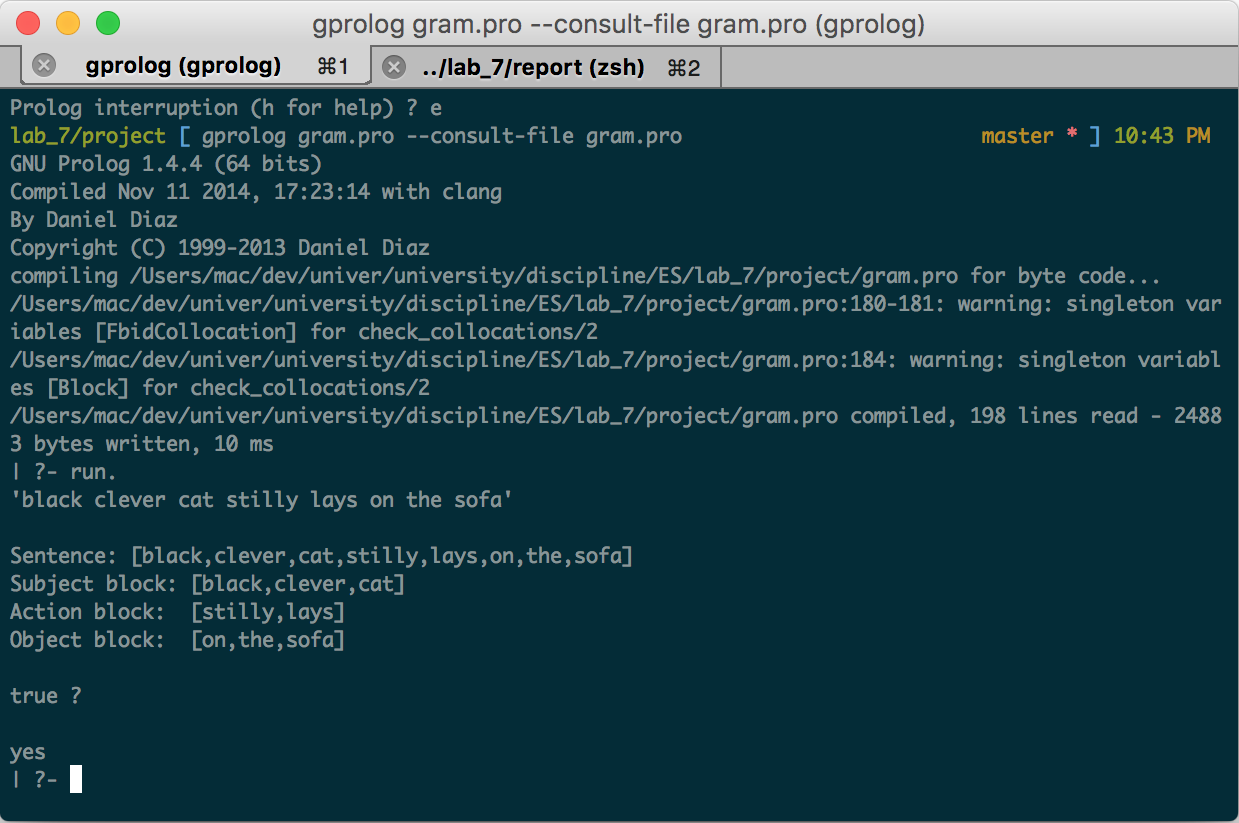
\includegraphics[width=130mm]{img/results}
  \caption{Результат работы программы}
  \label{fig:results}
\end{figure}

Исходный код программы расположен в приложении~А.

\newpage